\newcommand{\nom}{Porte conteneur}
\newcommand{\sequence}{03}
\newcommand{\num}{04}
\newcommand{\type}{TD}
\newcommand{\descrip}{Résolution d'un problème en utilisant des méthodes algorithmiques}
\newcommand{\competences}{Alt-C3: Concevoir un algorithme répondant à un problème précisément posé}
\documentclass[10pt,a4paper]{article}
  \usepackage[french]{babel}
  \usepackage[utf8]{inputenc}
  \usepackage[T1]{fontenc}
  \usepackage{xcolor}
  \usepackage[]{graphicx}
  \usepackage{makeidx}
  \usepackage{textcomp}
  \usepackage{amsmath}
  \usepackage{amssymb}
  \usepackage{stmaryrd}
  \usepackage{fancyhdr}
  \usepackage{lettrine}
  \usepackage{calc}
  \usepackage{boxedminipage}
  \usepackage[french,onelanguage, boxruled,linesnumbered]{algorithm2e}
  \usepackage[colorlinks=false,pdftex]{hyperref}
  \usepackage{minted}
  \usepackage{url}
  \usepackage[locale=FR]{siunitx}
  \usepackage{multicol}
  \usepackage{tikz}
  \makeindex

  %\graphicspath{{../Images/}}

%  \renewcommand\listingscaption{Programme}

  %\renewcommand{\thechapter}{\Alph{chapter}}
  \renewcommand{\thesection}{\Roman{section}}
  %\newcommand{\inter}{\vspace{0.5cm}%
  %\noindent }
  %\newcommand{\unite}{\ \textrm}
  \newcommand{\ud}{\mathrm{d}}
  \newcommand{\vect}{\overrightarrow}
  %\newcommand{\ch}{\mathrm{ch}} % cosinus hyperbolique
  %\newcommand{\sh}{\mathrm{sh}} % sinus hyperbolique

  \textwidth 160mm
  \textheight 250mm
  \hoffset=-1.70cm
  \voffset=-1.5cm
  \parindent=0cm

  \pagestyle{fancy}
  \fancyhead[L]{\bfseries {\large PTSI -- Dorian}}
  \fancyhead[C]{\bfseries{{\type} \no \numero}}
  \fancyhead[R]{\bfseries{\large Informatique}}
  \fancyfoot[C]{\thepage}
  \fancyfoot[L]{\footnotesize R. Costadoat, C. Darreye}
  \fancyfoot[R]{\small \today}
  
  \definecolor{bg}{rgb}{0.9,0.9,0.9}
  
  
  % macro Juliette
  
\usepackage{comment}   
\usepackage{amsthm}  
\theoremstyle{definition}
\newtheorem{exercice}{Exercice}
\newtheorem*{rappel}{Rappel}
\newtheorem*{remark}{Remarque}
\newtheorem*{defn}{Définition}
\newtheorem*{ppe}{Propriété}
\newtheorem{solution}{Solution}

\newcounter{num_quest} \setcounter{num_quest}{0}
\newcounter{num_rep} \setcounter{num_rep}{0}
\newcounter{num_cor} \setcounter{num_cor}{0}

\newcommand{\question}[1]{\refstepcounter{num_quest}\par
~\ \\ \parbox[t][][t]{0.15\linewidth}{\textbf{Question \arabic{num_quest}}}\parbox[t][][t]{0.85\linewidth}{#1\label{q\the\value{num_quest}}}\par
~\ \\}

\newcommand{\reponse}[4][1]
{\noindent
\rule{\linewidth}{.5pt}\\
\textbf{Question\ifthenelse{#1>1}{s}{} \multido{}{#1}{%
\refstepcounter{num_rep}\ref{q\the\value{num_rep}} }:} ~\ \\
\ifdef{\public}{#3 ~\ \\ \feuilleDR{#2}}{#4}
}

\newcommand{\cor}
{\refstepcounter{num_cor}
\noindent
\rule{\linewidth}{.5pt}
\textbf{Question \arabic{num_cor}:} \\
}


\usepackage{enumitem}

\setenumerate[1]{align=left,label=\arabic*}
\setenumerate[2]{before=\stepcounter{enumi},label*=.\arabic*,leftmargin=1.2em,align=left}


\ifdef{\public}{\excludecomment{solution}}


\begin{document}

\begin{center}
{\Large\bf {\type} \no {\numero} -- \descrip}
\end{center}

\SetKw{KwFrom}{de} 

\begin{boxedminipage}{.9\textwidth} 
\begin{itemize}
 \item Faire tous les exercices dans un même fichier {NomPrenom.py} à sauvegarder,
 \item Mettre en commentaire l'exercice et la question traités (ex: \# Exercice 1),
 \item Ne pas oublier pas de commenter ce qui est fait dans votre code (ex: \# Je crée une fonction pour calculer la racine d'un nombre),
 \item Il est possible de demander un déblocage pour certaines questions, mais celle-ci seront notées 0,
 \item Il faut vérifier avant de partir que le code peut s'exécuter et qu'il affiche les résultats que vous attendez. Les lignes de code qui doivent s'exécuter sont décommentées.
\end{itemize}
\end{boxedminipage}

\section*{Introduction}

Le but de ce travail est d'analyser un jeu de données des comptages horaires de vélos par compteur et localisation des sites de comptage. On se limitera pour des raisons de taille de fichier à la date du 11/11/2022.

Un compteur est un système placé sous la route comme le montre la figure \ref{img01} qui détecte le passage des vélos.

\begin{figure}[!ht]
\begin{center}
	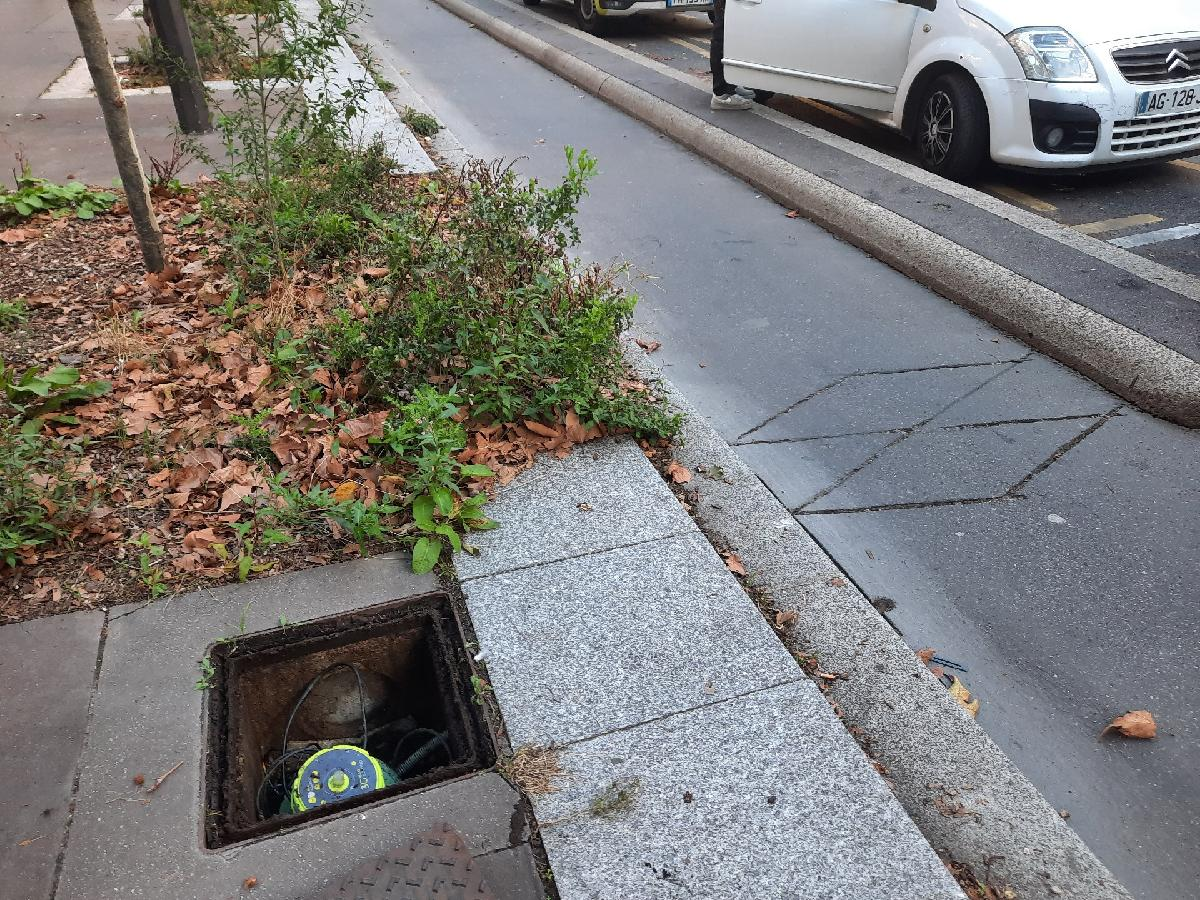
\includegraphics[width=0.5\linewidth]{img/compteur_daumesnil}
	\caption{Compteur installé sur la piste cyclable en bordure de l'avenue Daumesnil (75012).}
	\label{img01}
\end{center}
\end{figure}

Il peut être équipé d'un compteur dans le cas d'un aménagement cyclable unidirectionnel ou de deux compteurs dans le cas d'un aménagement cyclable bi-directionnel.

La Ville de Paris déploie depuis plusieurs années des compteurs vélo permanents pour évaluer le développement de la pratique cycliste.

Les compteurs sont situés sur des pistes cyclables et dans certains couloirs bus ouverts aux vélos. Les autres véhicules (ex : trottinettes,...) ne sont pas comptés.

Vous retrouverez ici :
\begin{itemize}
 \item Identifiant du compteur,
 \item Nom du compteur,
 \item Identifiant du site de comptage,
 \item Nom du site de comptage,
 \item Comptage horaire,
 \item Date et heure de comptage,
 \item La date d'installation du compteur,
 \item Les coordonnées GPS du compteur,
 \item La référence du compteur.
\end{itemize}    

Les données sont disponibles sur la page suivante:
\begin{center}
\url{https://www.data.gouv.fr/fr/datasets/comptage-velo-donnees-compteurs/}
\end{center}

\section{Analyse des données de comptage des passage de vélos dans les rues de Paris}

\subsection{Lecture du fichier de données}

Le fichier \verb?comptage-velo-donnees-compteurs_light.csv? présent dans le dossier \og /home/eleves/Ressources/PTSI/ \fg recense les données de comptage de l'ensemble des compteurs de la ville de Paris. 	

Pour cela nous allons dans un premier temps lire ce fichier en utilisant le code suivant.

\question{\textbf{Écrire} et \textbf{exécuter} un script permettant de lire le fichier de données et de découper son contenu sous la forme d'une liste \verb?lignes? dont chaque élément correspondra à une ligne du contenu sous la forme d'une chaîne de caractères (string).}

\textit{Remarque: Cette réponse étant nécessaire pour traiter la suite, il est autorisé de demander la correction à votre enseignant. La note à cette question sera alors de 0.}

Ainsi, \verb?ligne[0]? renvoi:\\
\verb?id_compteur;nom_compteur;id;name;sum_counts;date;installation_date;coordinates;counter;?

~\

Et \verb?ligne[1]? renvoi:\\
\verb?100003096-353242251;97 avenue Denfert Rochereau SO-NE;100003096;97 avenue Denfert?\\ \verb? Rochereau;6.0;2022-11-11T00:00:00+01:00;2012-02-22;48.83504,2.33314;X2H20012081;?

~\

Cela signifie que le compteur dont l'\verb?id? est \verb?100003096-353242251?, situé au \verb?97 avenue Denfert Rochereau? qui capte les vélos circulant dans le sens \verb?SO-NE? (sud-ouest vers nord-est), dont les coordonnées GPS sont \verb?48.83504,2.33314? (latitude, longitude) a vu passer \verb?6.0? vélos le \verb?2022-11-11? (11 novembre 2022) à \verb?T00:00:00+01:00? (entre 0h et 1h).

\begin{solution}~\ \\
\begin{minted}{python}
file_in=open('comptage-velo-donnees-compteurs_light.csv','r')
contenu=file_in.read()
file_in.close()
lignes=contenu.split('\n')
\end{minted}
\end{solution}

\subsection{Pic de circulation}

On souhaite savoir à quel moment de la journée ont lieu le plus de trajets en vélo. Pour cela, nous allons sommer pour chaque créneau horaire les données de l'ensemble des compteurs de la ville et enregistrer ces valeurs dans une liste \verb?creneaux?.


\question{\textbf{Recopier} et \textbf{compléter} le code suivant afin de générer la liste \verb?creneaux?.}

\begin{minted}{python}
creneaux=[0]*24

for ligne in lignes[1:-1]:
    data=ligne.split(';')
    creneaux[int(data[5][__:__])]+=float(_______)
print(creneaux)
\end{minted}

Ainsi, \verb?creneaux[0]? donne \verb?5631.0?, ce qui signifie qu'il y a 5631 passages de vélos sur les compteurs de toute la ville de Paris entre 0h et 1h du matin le 11/11/2022.

\begin{solution}~\ \\
\begin{minted}{python}
creneaux=[0]*24

for ligne in lignes[1:-1]:
    data=ligne.split(';')
    creneaux[int(data[5][11:13])]+=float(data[4])
print(creneaux)
\end{minted}
\end{solution}

Le code suivant permet de tracer les valeurs de \verb?creneaux? en fonction de l'heure.
\begin{minted}{python}
plt.plot(creneaux)
plt.show()
\end{minted}


\question{Grâce à cette commande, \textbf{déterminer} et \textbf{afficher} à l'aide d'un commentaire dans un \verb?print? l'heure à laquelle il y a eu un maximum de passages en vélo.}

\begin{solution}~\ \\
\begin{minted}{python}
plt.plot(creneaux)
plt.show()
print('Le max est de 10720 à 17h.')
\end{minted}

\verb?[5631.0, 3447.0, 2270.0, 1202.0, 954.0, 957.0, 1060.0, 1461.0, 2925.0, 4315.0, 5894.0, ?\\ \verb? 6450.0, 7489.0, 7345.0, 8244.0, 9880.0, 10643.0, 10720.0, 9610.0, 8801.0, 6487.0, 4297.0,?\\ \verb? 3789.0, 3810.0]?
\begin{center}
\resizebox{0.5\textwidth}{!}{%% Creator: Matplotlib, PGF backend
%%
%% To include the figure in your LaTeX document, write
%%   \input{<filename>.pgf}
%%
%% Make sure the required packages are loaded in your preamble
%%   \usepackage{pgf}
%%
%% Also ensure that all the required font packages are loaded; for instance,
%% the lmodern package is sometimes necessary when using math font.
%%   \usepackage{lmodern}
%%
%% Figures using additional raster images can only be included by \input if
%% they are in the same directory as the main LaTeX file. For loading figures
%% from other directories you can use the `import` package
%%   \usepackage{import}
%%
%% and then include the figures with
%%   \import{<path to file>}{<filename>.pgf}
%%
%% Matplotlib used the following preamble
%%   \usepackage{fontspec}
%%   \setmainfont{DejaVuSerif.ttf}[Path=\detokenize{/usr/share/matplotlib/mpl-data/fonts/ttf/}]
%%   \setsansfont{DejaVuSans.ttf}[Path=\detokenize{/usr/share/matplotlib/mpl-data/fonts/ttf/}]
%%   \setmonofont{DejaVuSansMono.ttf}[Path=\detokenize{/usr/share/matplotlib/mpl-data/fonts/ttf/}]
%%
\begingroup%
\makeatletter%
\begin{pgfpicture}%
\pgfpathrectangle{\pgfpointorigin}{\pgfqpoint{6.400000in}{4.800000in}}%
\pgfusepath{use as bounding box, clip}%
\begin{pgfscope}%
\pgfsetbuttcap%
\pgfsetmiterjoin%
\definecolor{currentfill}{rgb}{1.000000,1.000000,1.000000}%
\pgfsetfillcolor{currentfill}%
\pgfsetlinewidth{0.000000pt}%
\definecolor{currentstroke}{rgb}{1.000000,1.000000,1.000000}%
\pgfsetstrokecolor{currentstroke}%
\pgfsetdash{}{0pt}%
\pgfpathmoveto{\pgfqpoint{0.000000in}{0.000000in}}%
\pgfpathlineto{\pgfqpoint{6.400000in}{0.000000in}}%
\pgfpathlineto{\pgfqpoint{6.400000in}{4.800000in}}%
\pgfpathlineto{\pgfqpoint{0.000000in}{4.800000in}}%
\pgfpathlineto{\pgfqpoint{0.000000in}{0.000000in}}%
\pgfpathclose%
\pgfusepath{fill}%
\end{pgfscope}%
\begin{pgfscope}%
\pgfsetbuttcap%
\pgfsetmiterjoin%
\definecolor{currentfill}{rgb}{1.000000,1.000000,1.000000}%
\pgfsetfillcolor{currentfill}%
\pgfsetlinewidth{0.000000pt}%
\definecolor{currentstroke}{rgb}{0.000000,0.000000,0.000000}%
\pgfsetstrokecolor{currentstroke}%
\pgfsetstrokeopacity{0.000000}%
\pgfsetdash{}{0pt}%
\pgfpathmoveto{\pgfqpoint{0.800000in}{0.528000in}}%
\pgfpathlineto{\pgfqpoint{5.760000in}{0.528000in}}%
\pgfpathlineto{\pgfqpoint{5.760000in}{4.224000in}}%
\pgfpathlineto{\pgfqpoint{0.800000in}{4.224000in}}%
\pgfpathlineto{\pgfqpoint{0.800000in}{0.528000in}}%
\pgfpathclose%
\pgfusepath{fill}%
\end{pgfscope}%
\begin{pgfscope}%
\pgfsetbuttcap%
\pgfsetroundjoin%
\definecolor{currentfill}{rgb}{0.000000,0.000000,0.000000}%
\pgfsetfillcolor{currentfill}%
\pgfsetlinewidth{0.803000pt}%
\definecolor{currentstroke}{rgb}{0.000000,0.000000,0.000000}%
\pgfsetstrokecolor{currentstroke}%
\pgfsetdash{}{0pt}%
\pgfsys@defobject{currentmarker}{\pgfqpoint{0.000000in}{-0.048611in}}{\pgfqpoint{0.000000in}{0.000000in}}{%
\pgfpathmoveto{\pgfqpoint{0.000000in}{0.000000in}}%
\pgfpathlineto{\pgfqpoint{0.000000in}{-0.048611in}}%
\pgfusepath{stroke,fill}%
}%
\begin{pgfscope}%
\pgfsys@transformshift{1.025455in}{0.528000in}%
\pgfsys@useobject{currentmarker}{}%
\end{pgfscope}%
\end{pgfscope}%
\begin{pgfscope}%
\definecolor{textcolor}{rgb}{0.000000,0.000000,0.000000}%
\pgfsetstrokecolor{textcolor}%
\pgfsetfillcolor{textcolor}%
\pgftext[x=1.025455in,y=0.430778in,,top]{\color{textcolor}\sffamily\fontsize{10.000000}{12.000000}\selectfont 0}%
\end{pgfscope}%
\begin{pgfscope}%
\pgfsetbuttcap%
\pgfsetroundjoin%
\definecolor{currentfill}{rgb}{0.000000,0.000000,0.000000}%
\pgfsetfillcolor{currentfill}%
\pgfsetlinewidth{0.803000pt}%
\definecolor{currentstroke}{rgb}{0.000000,0.000000,0.000000}%
\pgfsetstrokecolor{currentstroke}%
\pgfsetdash{}{0pt}%
\pgfsys@defobject{currentmarker}{\pgfqpoint{0.000000in}{-0.048611in}}{\pgfqpoint{0.000000in}{0.000000in}}{%
\pgfpathmoveto{\pgfqpoint{0.000000in}{0.000000in}}%
\pgfpathlineto{\pgfqpoint{0.000000in}{-0.048611in}}%
\pgfusepath{stroke,fill}%
}%
\begin{pgfscope}%
\pgfsys@transformshift{2.005692in}{0.528000in}%
\pgfsys@useobject{currentmarker}{}%
\end{pgfscope}%
\end{pgfscope}%
\begin{pgfscope}%
\definecolor{textcolor}{rgb}{0.000000,0.000000,0.000000}%
\pgfsetstrokecolor{textcolor}%
\pgfsetfillcolor{textcolor}%
\pgftext[x=2.005692in,y=0.430778in,,top]{\color{textcolor}\sffamily\fontsize{10.000000}{12.000000}\selectfont 5}%
\end{pgfscope}%
\begin{pgfscope}%
\pgfsetbuttcap%
\pgfsetroundjoin%
\definecolor{currentfill}{rgb}{0.000000,0.000000,0.000000}%
\pgfsetfillcolor{currentfill}%
\pgfsetlinewidth{0.803000pt}%
\definecolor{currentstroke}{rgb}{0.000000,0.000000,0.000000}%
\pgfsetstrokecolor{currentstroke}%
\pgfsetdash{}{0pt}%
\pgfsys@defobject{currentmarker}{\pgfqpoint{0.000000in}{-0.048611in}}{\pgfqpoint{0.000000in}{0.000000in}}{%
\pgfpathmoveto{\pgfqpoint{0.000000in}{0.000000in}}%
\pgfpathlineto{\pgfqpoint{0.000000in}{-0.048611in}}%
\pgfusepath{stroke,fill}%
}%
\begin{pgfscope}%
\pgfsys@transformshift{2.985929in}{0.528000in}%
\pgfsys@useobject{currentmarker}{}%
\end{pgfscope}%
\end{pgfscope}%
\begin{pgfscope}%
\definecolor{textcolor}{rgb}{0.000000,0.000000,0.000000}%
\pgfsetstrokecolor{textcolor}%
\pgfsetfillcolor{textcolor}%
\pgftext[x=2.985929in,y=0.430778in,,top]{\color{textcolor}\sffamily\fontsize{10.000000}{12.000000}\selectfont 10}%
\end{pgfscope}%
\begin{pgfscope}%
\pgfsetbuttcap%
\pgfsetroundjoin%
\definecolor{currentfill}{rgb}{0.000000,0.000000,0.000000}%
\pgfsetfillcolor{currentfill}%
\pgfsetlinewidth{0.803000pt}%
\definecolor{currentstroke}{rgb}{0.000000,0.000000,0.000000}%
\pgfsetstrokecolor{currentstroke}%
\pgfsetdash{}{0pt}%
\pgfsys@defobject{currentmarker}{\pgfqpoint{0.000000in}{-0.048611in}}{\pgfqpoint{0.000000in}{0.000000in}}{%
\pgfpathmoveto{\pgfqpoint{0.000000in}{0.000000in}}%
\pgfpathlineto{\pgfqpoint{0.000000in}{-0.048611in}}%
\pgfusepath{stroke,fill}%
}%
\begin{pgfscope}%
\pgfsys@transformshift{3.966166in}{0.528000in}%
\pgfsys@useobject{currentmarker}{}%
\end{pgfscope}%
\end{pgfscope}%
\begin{pgfscope}%
\definecolor{textcolor}{rgb}{0.000000,0.000000,0.000000}%
\pgfsetstrokecolor{textcolor}%
\pgfsetfillcolor{textcolor}%
\pgftext[x=3.966166in,y=0.430778in,,top]{\color{textcolor}\sffamily\fontsize{10.000000}{12.000000}\selectfont 15}%
\end{pgfscope}%
\begin{pgfscope}%
\pgfsetbuttcap%
\pgfsetroundjoin%
\definecolor{currentfill}{rgb}{0.000000,0.000000,0.000000}%
\pgfsetfillcolor{currentfill}%
\pgfsetlinewidth{0.803000pt}%
\definecolor{currentstroke}{rgb}{0.000000,0.000000,0.000000}%
\pgfsetstrokecolor{currentstroke}%
\pgfsetdash{}{0pt}%
\pgfsys@defobject{currentmarker}{\pgfqpoint{0.000000in}{-0.048611in}}{\pgfqpoint{0.000000in}{0.000000in}}{%
\pgfpathmoveto{\pgfqpoint{0.000000in}{0.000000in}}%
\pgfpathlineto{\pgfqpoint{0.000000in}{-0.048611in}}%
\pgfusepath{stroke,fill}%
}%
\begin{pgfscope}%
\pgfsys@transformshift{4.946403in}{0.528000in}%
\pgfsys@useobject{currentmarker}{}%
\end{pgfscope}%
\end{pgfscope}%
\begin{pgfscope}%
\definecolor{textcolor}{rgb}{0.000000,0.000000,0.000000}%
\pgfsetstrokecolor{textcolor}%
\pgfsetfillcolor{textcolor}%
\pgftext[x=4.946403in,y=0.430778in,,top]{\color{textcolor}\sffamily\fontsize{10.000000}{12.000000}\selectfont 20}%
\end{pgfscope}%
\begin{pgfscope}%
\pgfsetbuttcap%
\pgfsetroundjoin%
\definecolor{currentfill}{rgb}{0.000000,0.000000,0.000000}%
\pgfsetfillcolor{currentfill}%
\pgfsetlinewidth{0.803000pt}%
\definecolor{currentstroke}{rgb}{0.000000,0.000000,0.000000}%
\pgfsetstrokecolor{currentstroke}%
\pgfsetdash{}{0pt}%
\pgfsys@defobject{currentmarker}{\pgfqpoint{-0.048611in}{0.000000in}}{\pgfqpoint{-0.000000in}{0.000000in}}{%
\pgfpathmoveto{\pgfqpoint{-0.000000in}{0.000000in}}%
\pgfpathlineto{\pgfqpoint{-0.048611in}{0.000000in}}%
\pgfusepath{stroke,fill}%
}%
\begin{pgfscope}%
\pgfsys@transformshift{0.800000in}{1.055877in}%
\pgfsys@useobject{currentmarker}{}%
\end{pgfscope}%
\end{pgfscope}%
\begin{pgfscope}%
\definecolor{textcolor}{rgb}{0.000000,0.000000,0.000000}%
\pgfsetstrokecolor{textcolor}%
\pgfsetfillcolor{textcolor}%
\pgftext[x=0.349316in, y=1.003116in, left, base]{\color{textcolor}\sffamily\fontsize{10.000000}{12.000000}\selectfont 2000}%
\end{pgfscope}%
\begin{pgfscope}%
\pgfsetbuttcap%
\pgfsetroundjoin%
\definecolor{currentfill}{rgb}{0.000000,0.000000,0.000000}%
\pgfsetfillcolor{currentfill}%
\pgfsetlinewidth{0.803000pt}%
\definecolor{currentstroke}{rgb}{0.000000,0.000000,0.000000}%
\pgfsetstrokecolor{currentstroke}%
\pgfsetdash{}{0pt}%
\pgfsys@defobject{currentmarker}{\pgfqpoint{-0.048611in}{0.000000in}}{\pgfqpoint{-0.000000in}{0.000000in}}{%
\pgfpathmoveto{\pgfqpoint{-0.000000in}{0.000000in}}%
\pgfpathlineto{\pgfqpoint{-0.048611in}{0.000000in}}%
\pgfusepath{stroke,fill}%
}%
\begin{pgfscope}%
\pgfsys@transformshift{0.800000in}{1.743979in}%
\pgfsys@useobject{currentmarker}{}%
\end{pgfscope}%
\end{pgfscope}%
\begin{pgfscope}%
\definecolor{textcolor}{rgb}{0.000000,0.000000,0.000000}%
\pgfsetstrokecolor{textcolor}%
\pgfsetfillcolor{textcolor}%
\pgftext[x=0.349316in, y=1.691217in, left, base]{\color{textcolor}\sffamily\fontsize{10.000000}{12.000000}\selectfont 4000}%
\end{pgfscope}%
\begin{pgfscope}%
\pgfsetbuttcap%
\pgfsetroundjoin%
\definecolor{currentfill}{rgb}{0.000000,0.000000,0.000000}%
\pgfsetfillcolor{currentfill}%
\pgfsetlinewidth{0.803000pt}%
\definecolor{currentstroke}{rgb}{0.000000,0.000000,0.000000}%
\pgfsetstrokecolor{currentstroke}%
\pgfsetdash{}{0pt}%
\pgfsys@defobject{currentmarker}{\pgfqpoint{-0.048611in}{0.000000in}}{\pgfqpoint{-0.000000in}{0.000000in}}{%
\pgfpathmoveto{\pgfqpoint{-0.000000in}{0.000000in}}%
\pgfpathlineto{\pgfqpoint{-0.048611in}{0.000000in}}%
\pgfusepath{stroke,fill}%
}%
\begin{pgfscope}%
\pgfsys@transformshift{0.800000in}{2.432080in}%
\pgfsys@useobject{currentmarker}{}%
\end{pgfscope}%
\end{pgfscope}%
\begin{pgfscope}%
\definecolor{textcolor}{rgb}{0.000000,0.000000,0.000000}%
\pgfsetstrokecolor{textcolor}%
\pgfsetfillcolor{textcolor}%
\pgftext[x=0.349316in, y=2.379319in, left, base]{\color{textcolor}\sffamily\fontsize{10.000000}{12.000000}\selectfont 6000}%
\end{pgfscope}%
\begin{pgfscope}%
\pgfsetbuttcap%
\pgfsetroundjoin%
\definecolor{currentfill}{rgb}{0.000000,0.000000,0.000000}%
\pgfsetfillcolor{currentfill}%
\pgfsetlinewidth{0.803000pt}%
\definecolor{currentstroke}{rgb}{0.000000,0.000000,0.000000}%
\pgfsetstrokecolor{currentstroke}%
\pgfsetdash{}{0pt}%
\pgfsys@defobject{currentmarker}{\pgfqpoint{-0.048611in}{0.000000in}}{\pgfqpoint{-0.000000in}{0.000000in}}{%
\pgfpathmoveto{\pgfqpoint{-0.000000in}{0.000000in}}%
\pgfpathlineto{\pgfqpoint{-0.048611in}{0.000000in}}%
\pgfusepath{stroke,fill}%
}%
\begin{pgfscope}%
\pgfsys@transformshift{0.800000in}{3.120182in}%
\pgfsys@useobject{currentmarker}{}%
\end{pgfscope}%
\end{pgfscope}%
\begin{pgfscope}%
\definecolor{textcolor}{rgb}{0.000000,0.000000,0.000000}%
\pgfsetstrokecolor{textcolor}%
\pgfsetfillcolor{textcolor}%
\pgftext[x=0.349316in, y=3.067420in, left, base]{\color{textcolor}\sffamily\fontsize{10.000000}{12.000000}\selectfont 8000}%
\end{pgfscope}%
\begin{pgfscope}%
\pgfsetbuttcap%
\pgfsetroundjoin%
\definecolor{currentfill}{rgb}{0.000000,0.000000,0.000000}%
\pgfsetfillcolor{currentfill}%
\pgfsetlinewidth{0.803000pt}%
\definecolor{currentstroke}{rgb}{0.000000,0.000000,0.000000}%
\pgfsetstrokecolor{currentstroke}%
\pgfsetdash{}{0pt}%
\pgfsys@defobject{currentmarker}{\pgfqpoint{-0.048611in}{0.000000in}}{\pgfqpoint{-0.000000in}{0.000000in}}{%
\pgfpathmoveto{\pgfqpoint{-0.000000in}{0.000000in}}%
\pgfpathlineto{\pgfqpoint{-0.048611in}{0.000000in}}%
\pgfusepath{stroke,fill}%
}%
\begin{pgfscope}%
\pgfsys@transformshift{0.800000in}{3.808283in}%
\pgfsys@useobject{currentmarker}{}%
\end{pgfscope}%
\end{pgfscope}%
\begin{pgfscope}%
\definecolor{textcolor}{rgb}{0.000000,0.000000,0.000000}%
\pgfsetstrokecolor{textcolor}%
\pgfsetfillcolor{textcolor}%
\pgftext[x=0.260951in, y=3.755522in, left, base]{\color{textcolor}\sffamily\fontsize{10.000000}{12.000000}\selectfont 10000}%
\end{pgfscope}%
\begin{pgfscope}%
\pgfpathrectangle{\pgfqpoint{0.800000in}{0.528000in}}{\pgfqpoint{4.960000in}{3.696000in}}%
\pgfusepath{clip}%
\pgfsetrectcap%
\pgfsetroundjoin%
\pgfsetlinewidth{1.505625pt}%
\definecolor{currentstroke}{rgb}{0.121569,0.466667,0.705882}%
\pgfsetstrokecolor{currentstroke}%
\pgfsetdash{}{0pt}%
\pgfpathmoveto{\pgfqpoint{1.025455in}{2.305126in}}%
\pgfpathlineto{\pgfqpoint{1.221502in}{1.553719in}}%
\pgfpathlineto{\pgfqpoint{1.417549in}{1.148771in}}%
\pgfpathlineto{\pgfqpoint{1.613597in}{0.781325in}}%
\pgfpathlineto{\pgfqpoint{1.809644in}{0.696000in}}%
\pgfpathlineto{\pgfqpoint{2.005692in}{0.697032in}}%
\pgfpathlineto{\pgfqpoint{2.201739in}{0.732469in}}%
\pgfpathlineto{\pgfqpoint{2.397787in}{0.870434in}}%
\pgfpathlineto{\pgfqpoint{2.593834in}{1.374124in}}%
\pgfpathlineto{\pgfqpoint{2.789881in}{1.852355in}}%
\pgfpathlineto{\pgfqpoint{2.985929in}{2.395611in}}%
\pgfpathlineto{\pgfqpoint{3.181976in}{2.586903in}}%
\pgfpathlineto{\pgfqpoint{3.378024in}{2.944372in}}%
\pgfpathlineto{\pgfqpoint{3.574071in}{2.894829in}}%
\pgfpathlineto{\pgfqpoint{3.770119in}{3.204130in}}%
\pgfpathlineto{\pgfqpoint{3.966166in}{3.766997in}}%
\pgfpathlineto{\pgfqpoint{4.162213in}{4.029508in}}%
\pgfpathlineto{\pgfqpoint{4.358261in}{4.056000in}}%
\pgfpathlineto{\pgfqpoint{4.554308in}{3.674104in}}%
\pgfpathlineto{\pgfqpoint{4.750356in}{3.395767in}}%
\pgfpathlineto{\pgfqpoint{4.946403in}{2.599633in}}%
\pgfpathlineto{\pgfqpoint{5.142451in}{1.846162in}}%
\pgfpathlineto{\pgfqpoint{5.338498in}{1.671384in}}%
\pgfpathlineto{\pgfqpoint{5.534545in}{1.678609in}}%
\pgfusepath{stroke}%
\end{pgfscope}%
\begin{pgfscope}%
\pgfsetrectcap%
\pgfsetmiterjoin%
\pgfsetlinewidth{0.803000pt}%
\definecolor{currentstroke}{rgb}{0.000000,0.000000,0.000000}%
\pgfsetstrokecolor{currentstroke}%
\pgfsetdash{}{0pt}%
\pgfpathmoveto{\pgfqpoint{0.800000in}{0.528000in}}%
\pgfpathlineto{\pgfqpoint{0.800000in}{4.224000in}}%
\pgfusepath{stroke}%
\end{pgfscope}%
\begin{pgfscope}%
\pgfsetrectcap%
\pgfsetmiterjoin%
\pgfsetlinewidth{0.803000pt}%
\definecolor{currentstroke}{rgb}{0.000000,0.000000,0.000000}%
\pgfsetstrokecolor{currentstroke}%
\pgfsetdash{}{0pt}%
\pgfpathmoveto{\pgfqpoint{5.760000in}{0.528000in}}%
\pgfpathlineto{\pgfqpoint{5.760000in}{4.224000in}}%
\pgfusepath{stroke}%
\end{pgfscope}%
\begin{pgfscope}%
\pgfsetrectcap%
\pgfsetmiterjoin%
\pgfsetlinewidth{0.803000pt}%
\definecolor{currentstroke}{rgb}{0.000000,0.000000,0.000000}%
\pgfsetstrokecolor{currentstroke}%
\pgfsetdash{}{0pt}%
\pgfpathmoveto{\pgfqpoint{0.800000in}{0.528000in}}%
\pgfpathlineto{\pgfqpoint{5.760000in}{0.528000in}}%
\pgfusepath{stroke}%
\end{pgfscope}%
\begin{pgfscope}%
\pgfsetrectcap%
\pgfsetmiterjoin%
\pgfsetlinewidth{0.803000pt}%
\definecolor{currentstroke}{rgb}{0.000000,0.000000,0.000000}%
\pgfsetstrokecolor{currentstroke}%
\pgfsetdash{}{0pt}%
\pgfpathmoveto{\pgfqpoint{0.800000in}{4.224000in}}%
\pgfpathlineto{\pgfqpoint{5.760000in}{4.224000in}}%
\pgfusepath{stroke}%
\end{pgfscope}%
\end{pgfpicture}%
\makeatother%
\endgroup%
}
\end{center}
\end{solution}

\newpage

\subsection{Créer la liste des compteurs}

Le code suivant permet de créer une liste \verb?compteurs? qui contient les données des compteurs qui nous intéressent, c'est à dire:
\begin{itemize}
 \item l'identifiant,
 \item le nom,
 \item les coordonnées GPS,
 \item le nombre de passage pour la journée (il sera pour le moment initialisé à 0).
\end{itemize}

\begin{minted}{python}
compteurs=[]
for ligne in lignes[1:-1]:
    data=ligne.split(';')
    if [data[0],data[1],data[7],0] not in compteurs:
        compteurs.append([data[0],data[1],[float(d) for d in data[7].split(',')],0])
\end{minted}

\question{\textbf{Écrire} le code permettant de déterminer et d'\textbf{afficher} le nombre de compteurs de la ville de Paris (un compteur bi-directionnel sera compté comme 2 compteurs). Valider votre code en vérifiant qu'il y en a plus de 2000.}

\begin{solution}~\ \\
\begin{minted}{python}
print(len(compteurs))
\end{minted}
Il y en a 2185.
\end{solution}

On souhaite maintenant modifier la valeur du nombre de passage pour chaque compteur de la liste \verb?compteurs? (pour le moment égale à 0).

~\

Pour cela, il est conseillé:
\begin{enumerate}
 \item De parcourir la liste \verb?lignes?,
 \item De découper chaque ligne à l'aide du séparateur ';',
 \item D'identifier pour chaque ligne, l'\verb?id? du compteur et de chercher le compteur correspondant dans la liste \verb?compteurs?,
 \item D'ajouter à la valeur du nombre de passage de chaque compteur de la liste \verb?compteurs?, la valeur du nombre de passage correspondant à la ligne de \verb?lignes?.
\end{enumerate}

\question{\textbf{Écrire} le code correspondant à ce pseudo code afin de modifier la liste \verb?compteurs? en conséquence.}

\textit{Remarque: Cette réponse étant nécessaire pour traiter la suite, il est autorisé de demander la correction à votre enseignant. La note à cette question sera alors de 0.}

\begin{solution}~\ \\
\begin{minted}{python}
for ligne in lignes[1:-1]:
    data=ligne.split(';')
    for compteur in compteurs:
        if compteur[0]==data[0]:
            compteur[3]+=float(data[4])
\end{minted}
\end{solution}

\section{Calcul de la distance entre deux compteurs}

On donne la fonction suivante qui permet de déterminer la distance (attention celle-ci n'est pas dans une unité SI) entre deux lieux dont les positions relatives sont caractérisées par deux listes \verb?lieu1? et \verb?lieu2? qui contiennent leur $latitude$ et $longitude$.

\begin{minted}{python}
def distance(lieu1, lieu2):
    return ((lieu1[0]-lieu2[0])**2+(lieu1[1]-lieu2[1])**2)**(1/2)
\end{minted}

Afin de rechercher les compteurs proches du lycée, celui-ci sera modélisé comme s'il s'agissait d'un compteur.

Ainsi, on écrira: \\ \verb?dorian=['0','74 Av. Philippe Auguste',[48.854576520866964, 2.3926308459105954],0]?

\question{\textbf{Écrire} le code permettant de déterminer et d'\textbf{afficher} la distance entre le lycée et le premier compteur de la liste \verb?compteurs?. Valider votre code en vérifiant que celle-ci est comprise entre $0.05$ et $0.1$.}

\begin{solution}~\ \\
\begin{minted}{python}
dorian=['0','74 Av. Philippe Auguste',[48.854576520866964, 2.3926308459105954],0]
print(distance(dorian[2],compteurs[0][2]))
\end{minted}
Le résultat est 0.06261658242625116
\end{solution}

\section{Recherche du plus gros hub à proximité}

\subsection{Recherche des 5 compteurs les plus proches}

Cette partie va consister en la recherche des 5 compteurs les plus proches d'un lieu.

Pour cela, on propose le pseudo-code suivant:
\begin{itemize}
 \item On crée une fonction \verb?get_five_more_close(depart)?,
 \item On part d'une distance \verb?d? nulle,
 \item On créer une liste \verb?five_more_close? vide,
 \item Tant que cette liste ne compte pas 5 éléments,
 \item On augmente la distance \verb?d? de $0.0001$,
 \item On cherche dans la liste \verb?compteurs? si un compteur est à une distance inférieure à \verb?d?.
 \item Si on en trouve un ET que ce n'est pas le \verb?depart? (\verb?!=?) ET qu'il n'est pas déjà dans la liste (\verb?not in?), on l'ajoute à \verb?five_more_close?
 \item On retourne \verb?five_more_close?
\end{itemize}

\question{\textbf{Écrire} le code correspondant à ce pseudo code. \textbf{Utiliser} cette fonction afin de \textbf{déterminer} et d'\textbf{afficher} les 5 plus proches éléments du lycée Dorian.}

\textit{Remarque: Cette réponse étant nécessaire pour traiter la suite, il est autorisé de demander la correction à votre enseignant. La note à cette question sera alors de 0.}

\begin{solution}~\ \\
\begin{minted}{python}
def get_five_more_close(depart):
    d=0
    five_more_close=[]
    while len(five_more_close)<5:
        d+=0.0001
        for compteur in compteurs:
            if distance(compteur[2],depart[2])<d and compteur not in five_more_close and compteur!=depart:
                five_more_close.append(compteur)
    return five_more_close

print(get_five_more_close(dorian))
\end{minted}
\end{solution}
  
\subsection{Recherche du plus gros hub}

On appelle \og plus gros hub\fg le compteur qui compte le plus de passage.

\question{\textbf{Écrire} une fonction getmax(compteurs) qui permet à partir d'une liste de compteurs de retourner celui qui compte le plus de passages.}

Ainsi, \verb?print(get_max(compteurs))? renvoie:\\
\verb?['100057445-104057445', 'Totem 73 boulevard de Sébastopol S-N', [48.86377, 2.35096], 6495.0]?

\begin{solution}~\ \\
\begin{minted}{python}
def getmax(compteurs):
    max=0
    for compteur in compteurs:
        if compteur[3]>max:
            max=compteur[3]
            plus_gros_hub=compteur
    return plus_gros_hub

print(get_max(compteurs))
\end{minted}
\end{solution}

\question{\textbf{Écrire} une commande permettant de déterminer le plus gros hub parmi les 5 plus proches du lycée Dorian.}

\begin{solution}~\ \\
\begin{minted}{python}
print(get_max(get_five_more_close(dorian)))
\end{minted}
\end{solution}

\section{Suivi d'un parcours de gros hub en gros hub}

Afin d'estimer l'itinéraire le plus emprunté à partir de Dorian, la suite va consister à
répéter \verb?n? fois les opérations suivantes, à partir d'un point de départ:
\begin{enumerate}
 \item sélectionner le compteur avec le plus de passage parmi les 5 plus proches,
 \item prendre ce compteur comme nouveau point de départ et ré-effectuer l'étape 1,
\end{enumerate}

\question{\textbf{Écrire} un algorithme qui effectuerait les opérations précédentes, avec \verb?n=10?.}

\begin{solution}~\ \\
\begin{minted}{python}
parcours=[dorian]
for i in range(10):
    parcours.append(get_max(get_five_more_close(parcours[i])))
print(parcours)
\end{minted}
\end{solution}

On constate que le parcours ainsi établit retombe plusieurs fois sur le même compteur (il faut \og demi-tour\fg).

\question{\textbf{Modifier} la fonction de la question 7 et l'algorithme de la question 10 afin de ne pas retomber deux fois sur le même compteur.}


\begin{solution}~\ \\
\begin{minted}{python}
def get_five_more_close_v2(hub,exclude):
    d=0
    five_more_close=[]
    while len(five_more_close)<5:
        d+=0.0001
        for compteur in compteurs:
            if distance(compteur[2],hub[2])<d and compteur not in five_more_close and compteur not in exclude:
                five_more_close.append(compteur)
    return five_more_close

parcours=[dorian]
for i in range(10):
    parcours.append(get_max(get_five_more_close_v2(parcours[i],parcours)))
print(parcours)
\end{minted}
\end{solution}

\end{document}


